% ======================================================
% Compile: xelatex aram_variance.tex
% Path:    reference/eq17_analysis/derivation/aram_variance.tex
% Derivation + simulation verification of the gain-fluctuation variance
%   Var(a_ram) = a'^2 * Var(delta_x)   (4-state AR(1), wall-normal axis).
% Base definitions mirror the Parameter model of 4state_del_hd_ar1.tex.
% Style mirrors 4state_del_hd_ar1 (monochrome, \fbox on key results, terse, math only).
% ======================================================
% fontset=none: no CJK text, do not load Chinese fonts.
\documentclass[11pt,a4paper,fontset=none]{ctexart}

\usepackage[fleqn]{amsmath}
\usepackage{amssymb,bm}
\usepackage{empheq}
\setlength{\mathindent}{0pt}
\usepackage{geometry}
\geometry{margin=2.0cm}
\usepackage{enumitem}
\usepackage{array,booktabs}
\usepackage{titlesec}
\usepackage{graphicx}

\setlength{\parindent}{0pt}
\setlength{\parskip}{0.3em}
\setlength{\abovedisplayskip}{4pt}
\setlength{\belowdisplayskip}{4pt}
\setlength{\abovedisplayshortskip}{2pt}
\setlength{\belowdisplayshortskip}{2pt}

\newcommand{\lc}{\lambda_c}
\newcommand{\hd}[1]{\par\medskip\noindent\underline{\textbf{#1}}\par\nobreak\vspace{0.2ex}}

\begin{document}

\hd{Parameter model}
\[ a_x[k] = a_{x_{det}}[k] + a_{x_{ram}}[k]; \qquad a_{x_{ram}}[k] \approx a'_x[k]\, x_{ram}[k] \]
\[ a'_x := \frac{d a_x}{d h} = -\frac{a_x K_h}{R}, \qquad K_h = \frac{1}{c}\frac{dc}{d\bar h} \]
\textbf{Assumption} ($x = x_{det}+x_{ram}$, $x_{det}=x_d$): $\;\delta x = x_d - x = -x_{ram}$, $\;\delta h = (x-x_d)\cdot\hat w = -\delta x$.
\[ a_{x_{ram}} = a_x(h_d+\delta h) - a_x(h_d) = a'_x\,\delta h + O\!\big(\tfrac12 a''_x\,\delta h^2\big) \]
\begin{empheq}[box=\fbox]{equation*}
a_{x_{ram}} = a'_x\, x_{ram} = -a'_x\,\delta x
\end{empheq}

\hd{Gain-fluctuation variance}
\begin{empheq}[box=\fbox]{equation*}
\mathrm{Var}(a_{x_{ram}}) = a'^2_x\,\mathrm{Var}(x_{ram}) = a'^2_x\,\mathrm{Var}(\delta x) \qquad (1)
\end{empheq}
\textbf{Closed-loop} ($\delta x[k+1]=\lc\,\delta x[k]-\varepsilon[k]$, $\hat a_x=a_x$):
\[ \mathrm{Var}(\delta x) = C_{\delta x}\,\sigma^2_{\delta h}, \qquad C_{\delta x} = 2 + \frac{1}{1-\lc^2}, \qquad \sigma^2_{\delta h} := 4 k_B T\, a_\perp \]
\textbf{Measurement} ($\delta x_m = \delta x[k-d] + n_x$): $\;\mathrm{Var}(\delta x_m) = \mathrm{Var}(\delta x) + \sigma^2_n$.
\begin{empheq}[box=\fbox]{equation*}
\mathrm{Var}(a_{x_{ram}}) = a'^2_x\,\big(\mathrm{Var}(\delta x_m) - \sigma^2_n\big) \qquad (2)
\end{empheq}
\textbf{Explicit} ($a'^2_x = a_x^2 K_h^2 / R^2$):
\begin{empheq}[box=\fbox]{equation*}
\mathrm{Var}(a_{x_{ram}}) = C_{\delta x}\,4 k_B T\,\frac{K_h^2\, a_x^3}{R^2} \qquad (3)
\end{empheq}

\hd{Verification} (1\,Hz, near wall, cross-seed ensemble; 4-state AR(1); $z$; $N=100$)
\[ \delta x[k] = x_d[k] - x[k-1] \]

\medskip
\noindent\begin{minipage}{\linewidth}\centering
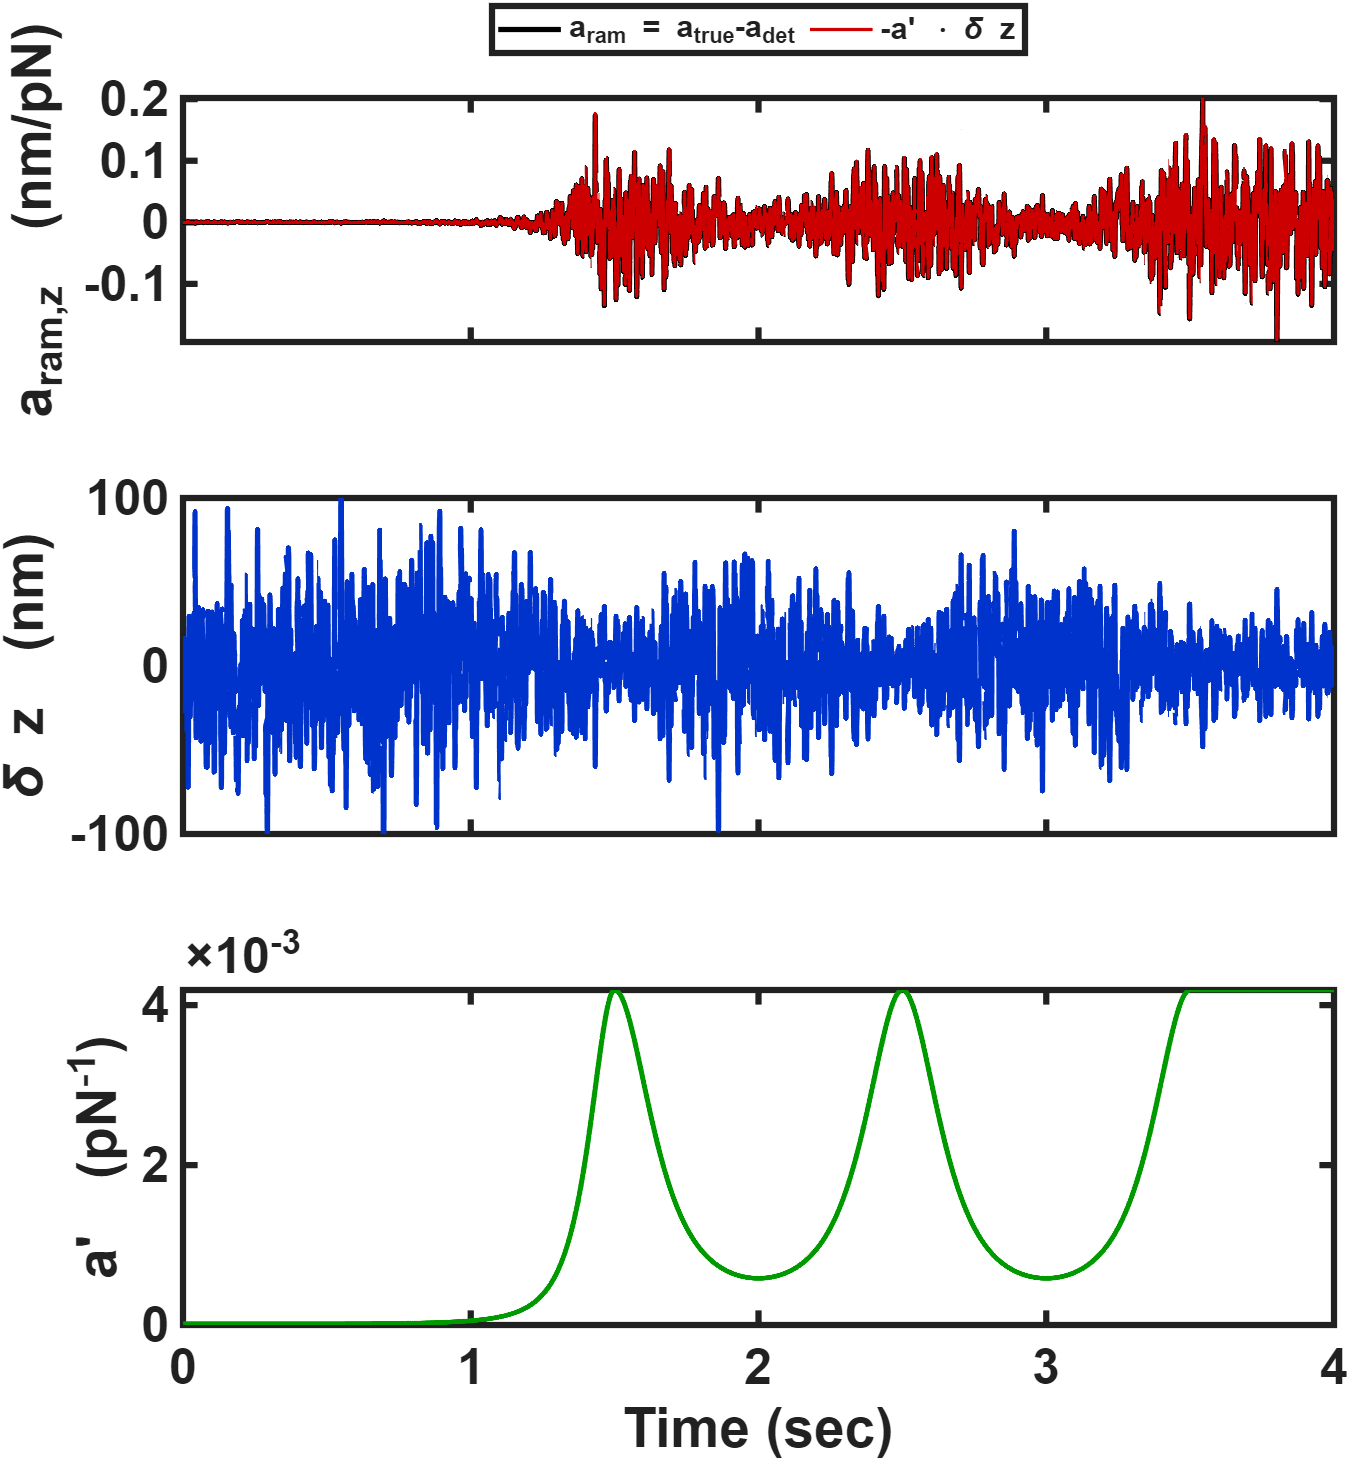
\includegraphics[width=0.62\textwidth]{figures/aram_signals.png}\\[0.4ex]
{\small $a_{ram}=a_{true}-a_{det}$ and $-a'\,\delta z$ (top); $\delta z$ (middle); $a'$ (bottom).}
\end{minipage}

\medskip
\noindent\begin{minipage}{\linewidth}\centering
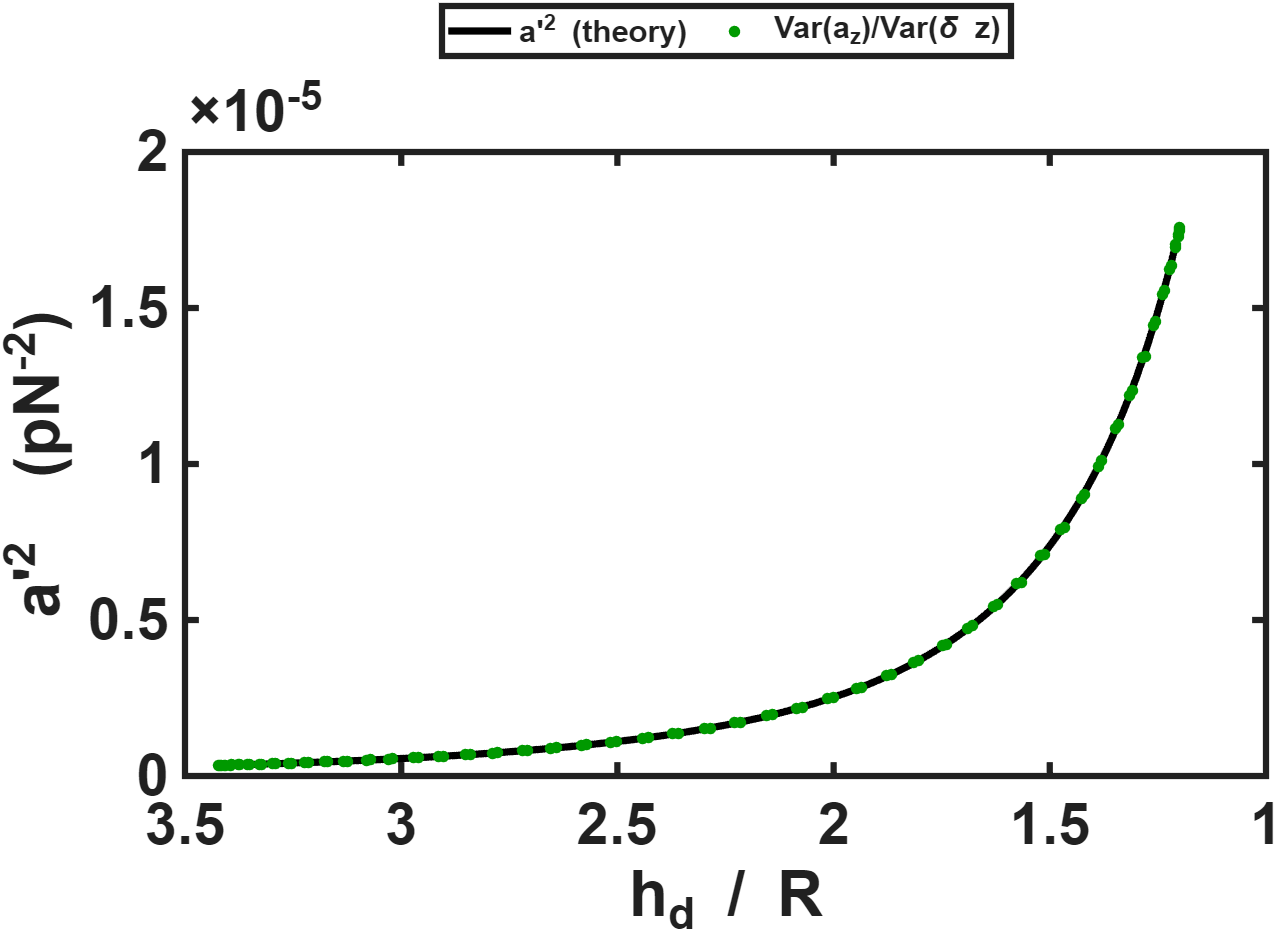
\includegraphics[width=0.74\textwidth]{figures/aram_ratio.png}\\[0.4ex]
{\small $\mathrm{Var}(a_z)/\mathrm{Var}(\delta z)$ vs $a'^2(\bar h)$ \quad (form 1).}
\end{minipage}

\medskip
\noindent\begin{minipage}{\linewidth}\centering
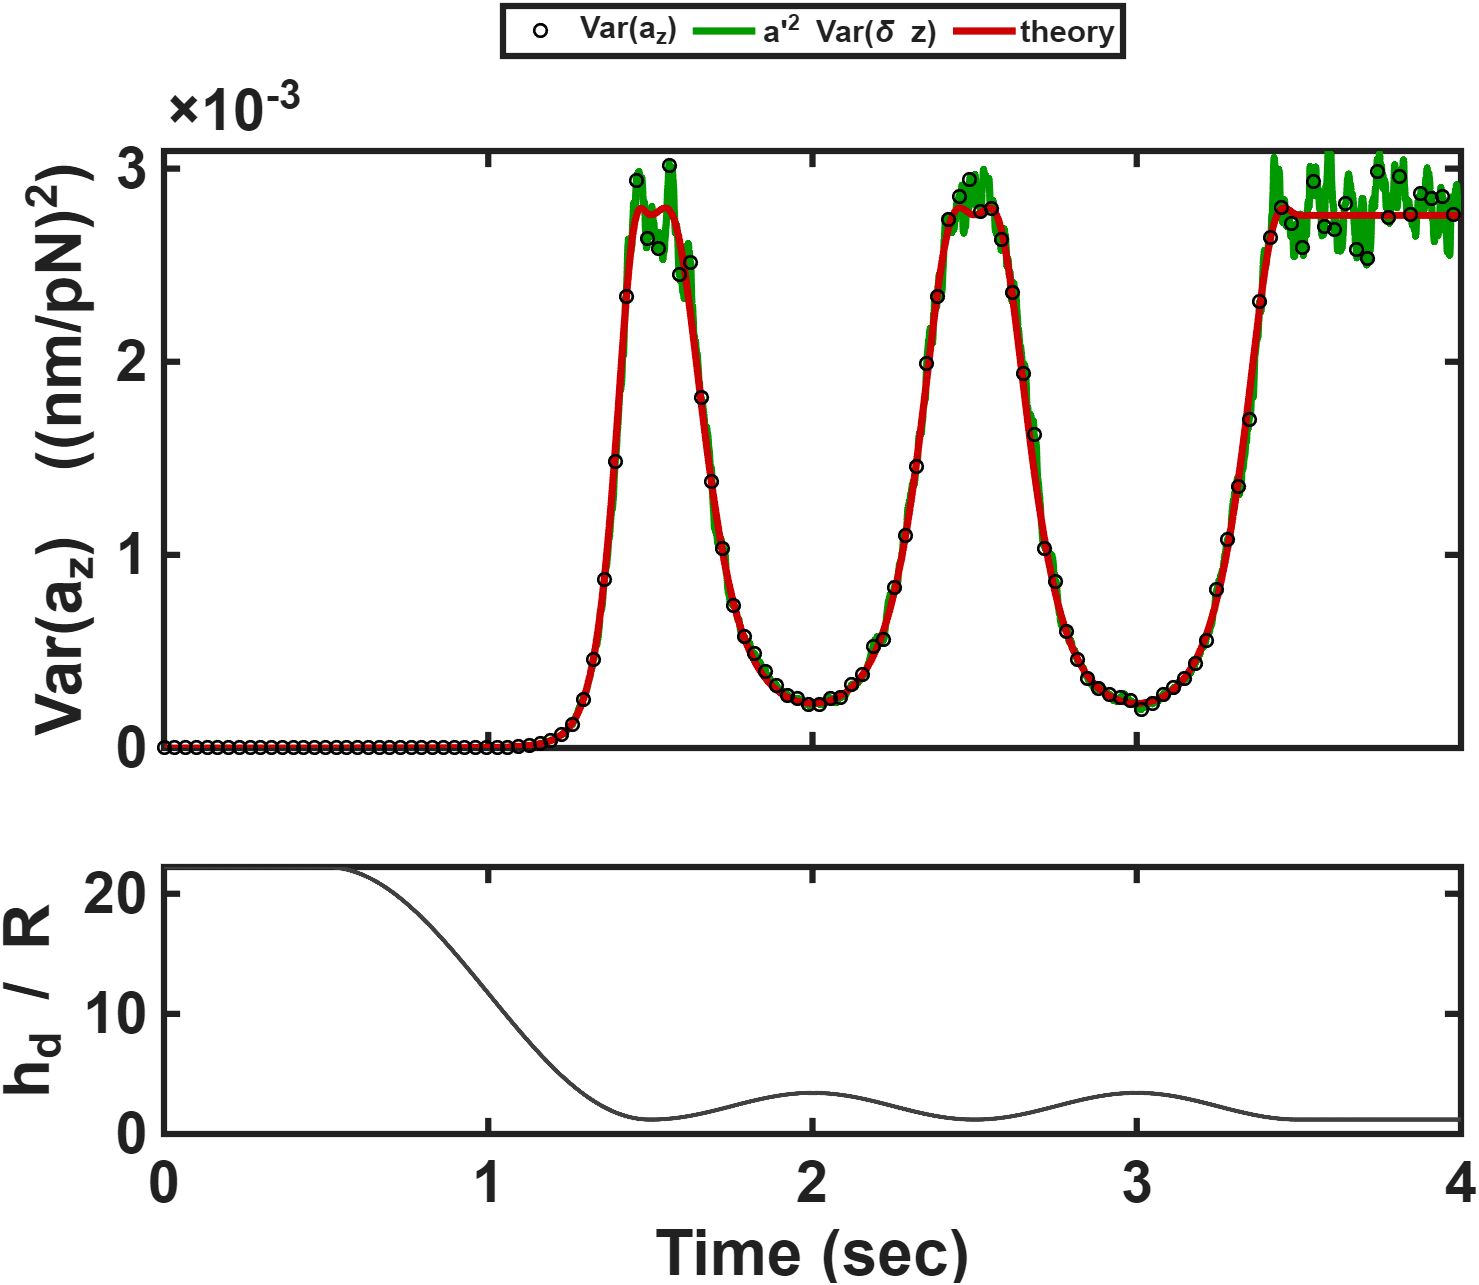
\includegraphics[width=0.82\textwidth]{figures/aram_absvar.png}\\[0.4ex]
{\small $\mathrm{Var}(a_z)$: measured, $a'^2\,\mathrm{Var}(\delta z)$ (1), $C_{\delta x}4k_BT K_h^2 a_z^3/R^2$ (3); $h_d/R$ below.}
\end{minipage}

\end{document}
